\documentclass[11pt,a4paper]{article}
\usepackage[utf8]{inputenc}
\usepackage[T1]{fontenc}
\usepackage[margin=2cm]{geometry}
\usepackage{amsmath,amssymb}
\usepackage{tikz}

\pagestyle{empty}

\begin{document}
	
	\begin{center}
		\large\textbf{Práctica 3: Cuestiones}
	\end{center}
	\vspace{0.2cm}
	
	% --- CUESTIÓN 1 ---
	\textbf{Cuestión 1.} \textit{Determine el valor de $R_L$ que asegura el funcionamiento del circuito.}
	
	Para no superar la corriente directa máxima admisible ($I_{FAV}$) del diodo:
	\[
	I_{\text{max}} = \frac{V_{e,\text{pico}} - V_\gamma}{R_L} \le I_{FAV} \implies R_L \ge \frac{V_{e,\text{pico}} - V_\gamma}{I_{FAV}}
	\]
\begin{itemize}
	\item Para diodo \textbf{1N4007} ($I_{FAV} = 1\text{ A}$, $V_\gamma \approx 0.7\text{ V}$, $V_{e,\text{pico}} = 5\text{ V}$):
	\[
	R_L \ge \frac{5 - 0.7}{1} = \mathbf{4.3\,\Omega}
	\]
	\item Para diodo \textbf{1N4148} ($I_{FAV} = 200\text{ mA}$): 
	\[
	R_L \ge \frac{5 - 0.7}{0.2} = \mathbf{21.5\,\Omega}
	\]
\end{itemize}
	Con la resistencia montada en el circuito ($R_1 = 1\text{ k}\Omega$), la corriente de pico es de aprox. $4.3\text{ mA}$, garantizando un funcionamiento totalmente seguro.
	
	\vspace{0.4cm}
	
	% --- CUESTIÓN 2 ---
	\textbf{Cuestión 2.} \textit{Represente la función de transferencia del rectificador de media onda.}
	
	\begin{minipage}{0.55\textwidth}
		\[
		v_s = \begin{cases} 
			0\text{ V}, & v_e \le V_\gamma \ (\approx 0.7\text{ V}) \\ 
			v_e - V_\gamma, & v_e > V_\gamma 
		\end{cases}
		\]
	\end{minipage}
	\hfill
	\begin{minipage}{0.4\textwidth}
		\centering
		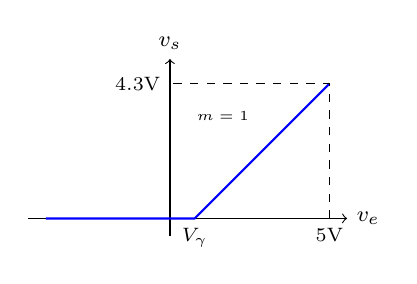
\begin{tikzpicture}[scale=0.45]
			\draw[->] (-4,0) -- (5,0) node[right] {\footnotesize $v_e$};
			\draw[->] (0,-0.5) -- (0,4.5) node[above] {\footnotesize $v_s$};
			\draw[thick, blue] (-3.5,0) -- (0.7,0) -- (4.5,3.8);
			\draw[dashed] (0.7,0) node[below] {\scriptsize $V_\gamma$} -- (0.7,0);
			\draw[dashed] (4.5,0) node[below] {\scriptsize $5\text{V}$} -- (4.5,3.8) -- (0,3.8) node[left] {\scriptsize $4.3\text{V}$};
			\node at (2.5,2.5) [above left] {\tiny $m=1$};
		\end{tikzpicture}
	\end{minipage}
	
	\vspace{0.4cm}
	
	% --- CUESTIÓN 3 ---
	\textbf{Cuestión 3.} \textit{Represente la función de transferencia del circuito recortador.}
	
	\begin{minipage}{0.55\textwidth}
		\[
		v_s = \begin{cases} 
			-V_\gamma \approx -0.7\text{ V}, & v_e < -V_\gamma \ (D_2 \text{ ON}) \\ 
			v_e, & -V_\gamma \le v_e \le V_{DD} + V_\gamma \\ 
			V_{DD} + V_\gamma \approx 5.7\text{ V}, & v_e > V_{DD} + V_\gamma \ (D_1 \text{ ON})
		\end{cases}
		\]
	\end{minipage}
	\hfill
	\begin{minipage}{0.4\textwidth}
		\centering
		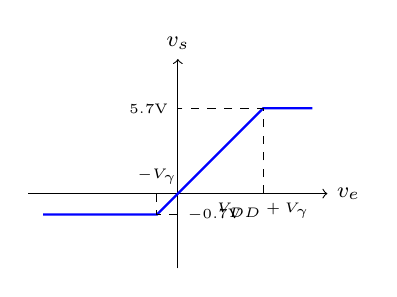
\begin{tikzpicture}[scale=0.38]
			\draw[->] (-5,0) -- (5,0) node[right] {\footnotesize $v_e$};
			\draw[->] (0,-2.5) -- (0,4.5) node[above] {\footnotesize $v_s$};
			\draw[thick, blue] (-4.5,-0.7) -- (-0.7,-0.7) -- (2.85,2.85) -- (4.5,2.85);
			\draw[dashed] (-0.7,0) node[above] {\tiny $-V_\gamma$} -- (-0.7,-0.7) -- (0,-0.7) node[right] {\tiny $-0.7\text{V}$};
			\draw[dashed] (2.85,0) node[below] {\tiny $V_{DD}+V_\gamma$} -- (2.85,2.85) -- (0,2.85) node[left] {\tiny $5.7\text{V}$};
		\end{tikzpicture}
	\end{minipage}
	
	\vspace{0.4cm}
	
	% --- CUESTIÓN 4 ---
	\textbf{Cuestión 4.} \textit{Represente la señal de entrada y de salida del rectificador de precisión para una señal sinusoidal de $10\text{ V}$ de amplitud.}
	
	\begin{minipage}{0.55\textwidth}
		\begin{itemize}
			\item Para $v_e > 0$: $v_L = 0\text{ V}$.
			\item Para $v_e < 0$: $v_L = -\left(\frac{R_2}{R_1}\right)v_e = -2\,v_e$.
		\end{itemize}
		Con amplitud de pico $10\text{ V}$, la salida teórica buscaría un pico de $+20\text{ V}$. 
		
		Sin embargo, como el AO está alimentado con $\pm 10\text{ V}$ ($V_{CC} = +10\text{ V}$), \textbf{la señal se satura} en torno a $V_{\text{sat}}^+ \approx 8.5\text{ V} - 9.0\text{ V}$ (o $10\text{ V}$ ideal), recortando la cresta.
	\end{minipage}
	\hfill
	\begin{minipage}{0.4\textwidth}
		\centering
		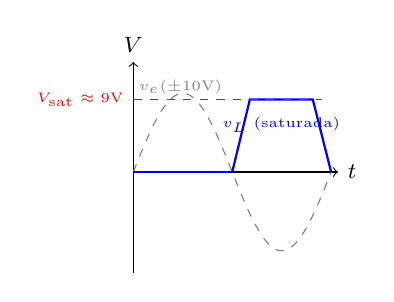
\begin{tikzpicture}[scale=0.4]
			\draw[->] (0,0) -- (6.5,0) node[right] {\footnotesize $t$};
			\draw[->] (0,-3.2) -- (0,3.5) node[above] {\footnotesize $V$};
			% v_e
			\draw[domain=0:6.28, samples=50, smooth, gray, dashed] plot (\x, {2.5*sin(\x r)});
			\node[gray] at (1.5,2.7) {\tiny $v_e (\pm 10\text{V})$};
			% v_L
			\draw[thick, blue] (0,0) -- (3.14,0);
			\draw[thick, blue] (3.14,0) -- (3.7, 2.3) -- (5.7, 2.3) -- (6.28, 0);
			\draw[dashed, red] (0,2.3) node[left] {\tiny $V_{\text{sat}} \approx 9\text{V}$} -- (6,2.3);
			\node[blue] at (4.7,1.5) {\tiny $v_L$ (saturada)};
		\end{tikzpicture}
	\end{minipage}
	
\end{document}